\chapter{Sample Retrieval Lander Class Assessment}\label{Ch:SRL_EDL}
In Ref.~\cite{MyRobustOCPaper}, an earlier version of the work in the dissertation, we assessed the robust optimal guidance on a vehicle in the class of the Sample Retrieval Lander (SRL) mission of the Mars Sample Return campaign\cite{MSR,MSR2}. The ballistic coefficient of the vehicle is 200 $ \mathrm{kg/m}^2 $ with an entry mass of 5000 kg. In order to contend with the increased ballistic coefficient, the vehicle L/D is raised to 0.28 (assumed to be constant, in contrast to the earlier results for the MSL-class vehicle). The same state and uncertainty at the entry interface presented in Chapter~\ref{Ch:AssessmentConditions} are assumed. The resulting mean entry state is $x_0 = [54.5\,\mathrm{km},\,-11.5^{\circ}, 0\,\mathrm{km}]^T$ at $v_0 = 5525$ m/s. The same parametric uncertainty is considered except the altitude-varying Mars Climate Database model is replaced with a constant fractional offset with $3\sigma_{\rho} = 20$\%. In this earlier work, we had not yet developed the DDP extension to jointly optimize the static feedback gains presented in Section~\ref{Sec:DesignOptimization}. As a result, any feedback gain optimization presented in this chapter was performed separately from the reference control using a sequential quadratic programming method to minimize the original terminal objective in Eq.~\eqref{Eq:Objective}, as estimated using the UT.

In the first section, the unscented transform is used to estimate the performance of an unguided entry vehicle to determine the magnitude of errors that must be mitigated by the entry guidance. In the second section, reference trajectories and controls generated by our approach are compared to those designed by nominal optimal control with fixed bank angle margins. By nominal optimal control we refer to the optimization of a single trajectory without considering uncertainty or closed-loop guidance. The third section investigates how the optimal trajectories change with the weights $w_h$ and $w_s$, incorporating both initial state uncertainty and parametric uncertainty. The final subsection presents a detailed look at one solution and the corresponding Monte Carlo statistics.

\section{Open-Loop Simulation}
\begin{figure}[h!]
	\centering
	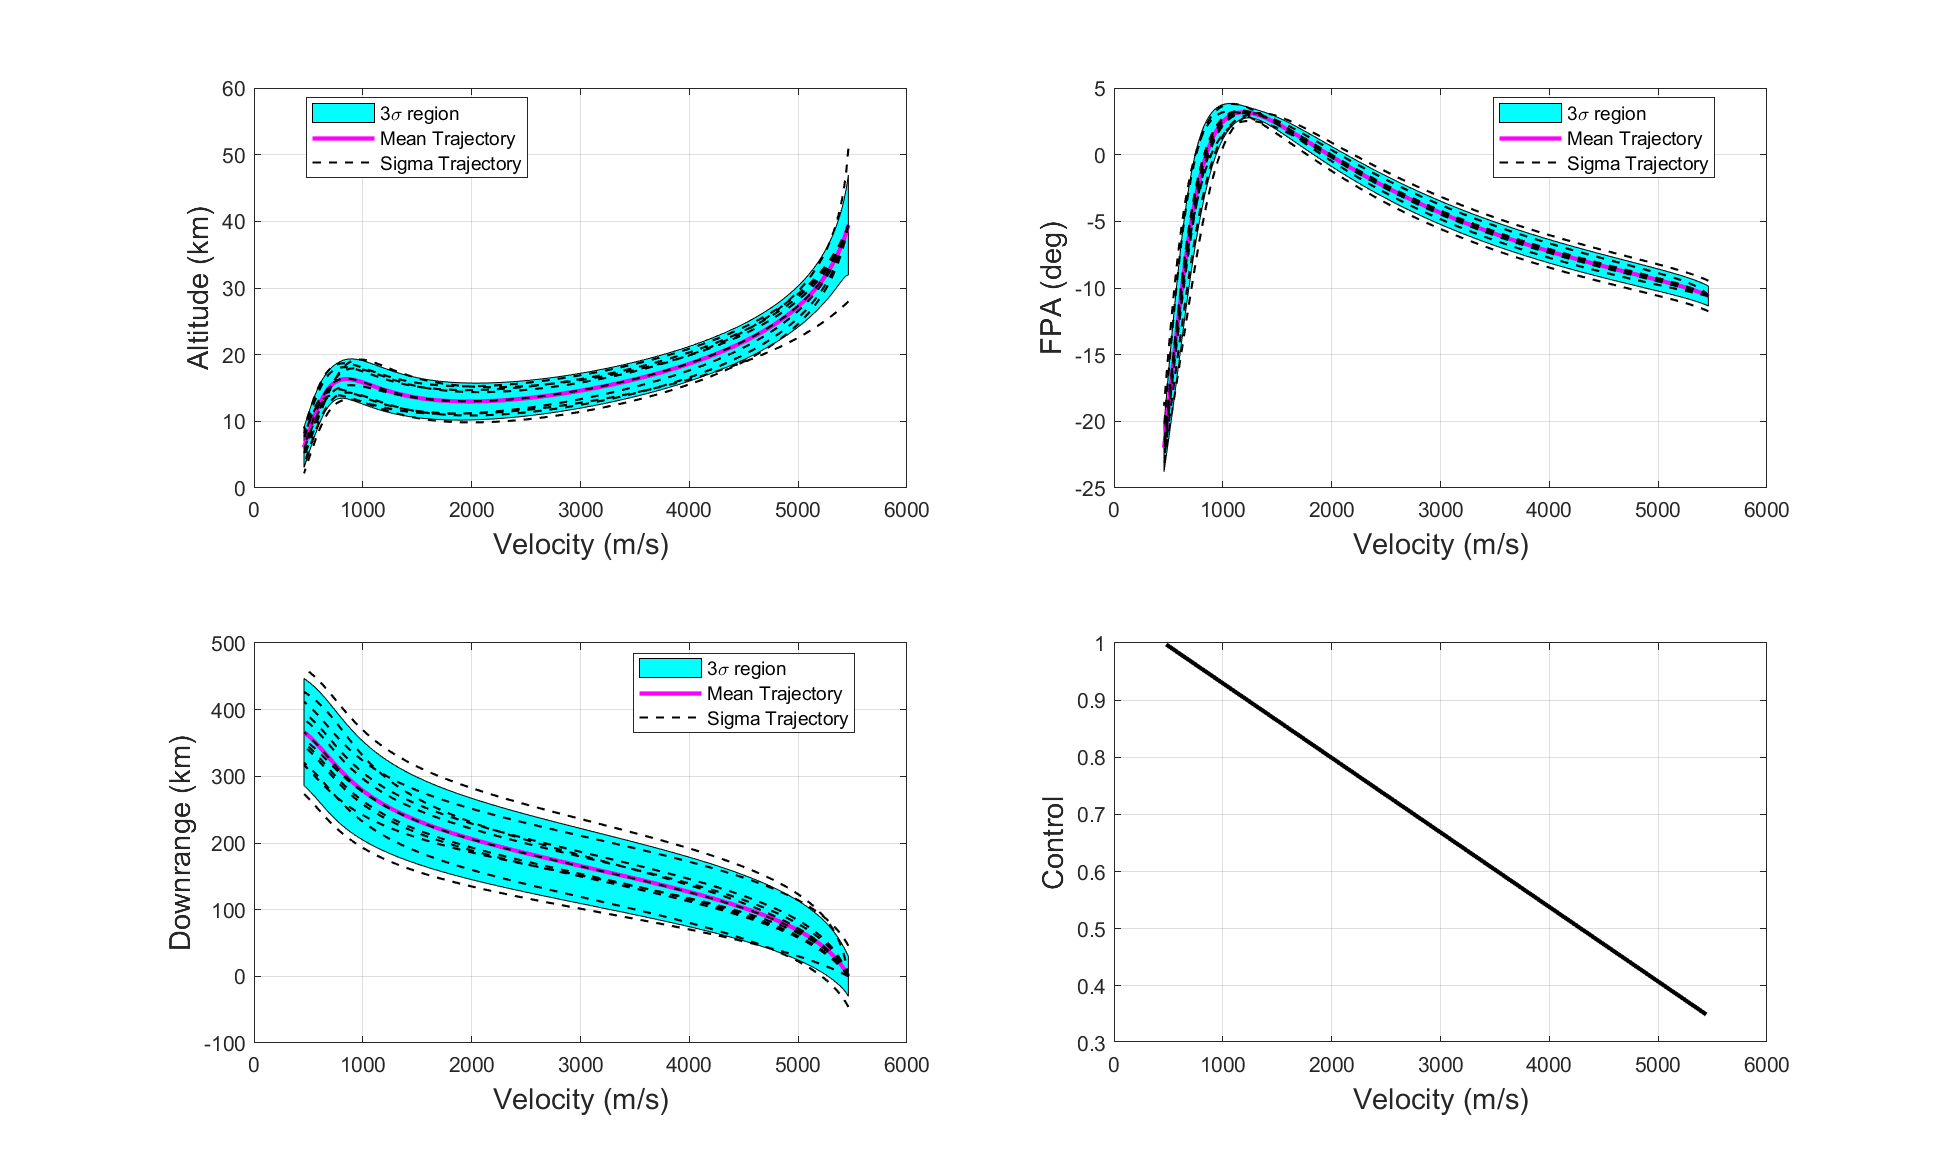
\includegraphics[width=1\textwidth]{../PropellantOptimalJournal/ddp/matlab/HeavyOpenLoopGrid}
	\caption{The sigma point trajectories for an unguided entry trajectory.}
	\label{Fig:OpenLoop}
\end{figure}
In order to estimate the magnitude of the range and altitude dispersions that must be mitigated by the guidance commands, we simulate the performance of our initial trajectory with the feedback gains set to zero. Since the purpose of determining the magnitude of the terminal errors is as a point of reference, the unscented transform estimate is used rather than full Monte Carlo simulation. The altitude, range, FPA, and nominal control profiles are shown in Fig.~\ref{Fig:OpenLoop}, including the sigma point trajectories and the UT-estimated 3$\sigma$ region. The control profile, shown in the bottom right of the figure, is a linear ramp from $u(v_0)=0.35$ to $ u(v_f)=1 $. The mean altitude is 6.08 km and the 3$\sigma$-low altitude is 3.09 km. At the chute deploy velocity, 460 m/s, the target range is 366.4 km and the 3$\sigma$ range error is $80.3$ km. Thus the robust optimal guidance has substantial potential errors to overcome.

\section{Reference Trajectory Comparison}
In this subsection we compare the performance of the robust optimal guidance using six different reference trajectory-control pairs. For all six cases, the control law in Eq.~(\ref{Eq:Control}) is used with the same feedback gains and feedback control limits, Eq.~(\ref{Eq:Control_bounds}). In the first three cases, a reference trajectory and control are generated by solving the optimal control problem $\min J = -h(v_f)$ subject to nominal longitudinal dynamics with different limits on the reference control to preserve margin for feedback. For the remaining three cases, the solution to the ROGP is used to generate the reference trajectory and control. Monte Carlo simulations are used to assess the guidance performance.

Case 1 considers $u_{\mathrm{ref}}\in[0,1] = [\cos90^{\circ},\cos0^{\circ}]$, Case 2 considers $u_{\mathrm{ref}}\in [\cos75^{\circ},\cos15^{\circ}]$, and Case 3 considers $u_{\mathrm{ref}}\in [\cos60^{\circ},\cos30^{\circ}]$.
Bank angle margin is important for range control, as well as for preserving control authority for lateral guidance, which is not modeled here. 
Cases 4-6 solve the robust optimal guidance problem with different choices of the weights to design the reference trajectories. Case 4 optimizes mean altitude ($ w_h=w_s=0 $), Case 5 optimizes the 3$\sigma$-low altitude ($ w_h=3,\,w_s=0 $), and Case 6 optimizes a combination of mean altitude and 3$\sigma$ downrange deviation ($ w_h=0, w_s=3 $). Recall that each of the six cases may achieve a different downrange distance.

The feedback gains are constants $[k_D, k_{\gamma}, k_s] = [0.0725, -0.025, -0.004]$.  These gains were computed by minimizing the UT-estimated downrange distance standard deviation for the initial guess at the control profile, which is a linear (in velocity) ramp from zero to one. Different initial guesses for the optimal profile would yield some variation in these gains, and superior results can be obtained by optimizing the gains for each solution, but using the same gains for all of the cases allows us to highlight the impact of the reference trajectory without confounding variables. These gains are used in the optimization process for Cases 4-6, and in the Monte Carlo simulations for all six cases. 

\begin{figure}[h!]
	\centering
	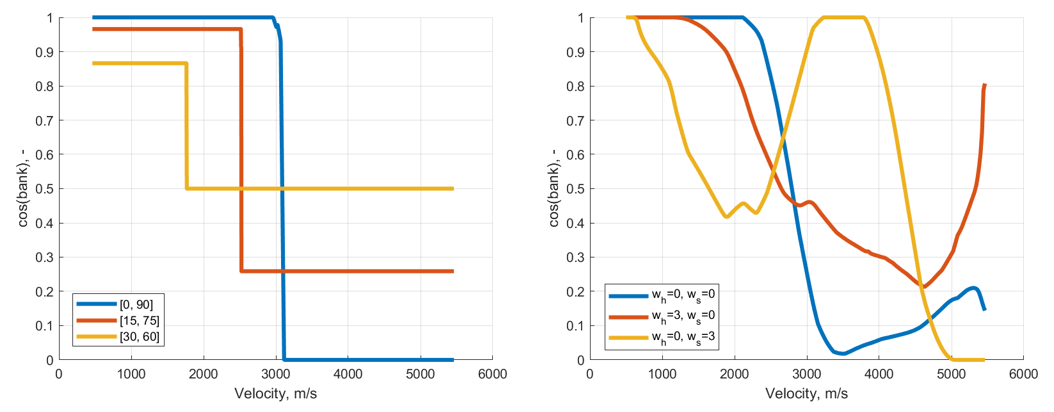
\includegraphics[width=1\textwidth]{../PropellantOptimalJournal/ddp/comparison_controls}
	\caption{The profiles from deterministic optimal control (left) exhibit the well known bang-bang structure of altitude optimal trajectories. In comparison, the robust control histories (right) exhibit significantly different behavior depending on the weights applied.}
	\label{fig_control_comparison}
\end{figure}

Figure~\ref{fig_control_comparison} shows the resulting control profiles for the six cases. The altitude-optimal controls resulting from nominal optimal control (Cases 1-3) exhibit the well-known bang-bang structure, while the robust optimal control profiles are quite varied depending on the weights selected. For Case 4, which optimizes mean altitude, the profile is somewhat similar to the bang-bang profiles, but retains margin at high velocities and has a slower transition to a lift up ($u=1$) orientation. An interesting feature of the robust profiles is that they exhibit significant margins, as solutions to the problem that considers robustness. Nevertheless, saturation still occurs at some velocities. This suggests that the robust optimal amount of margin varies along the trajectory, which implies using a fixed margin will produce inferior results, as the results presented next indicate. Although lateral guidance control authority ($L/D \sin\sigma$) is not considered in the formulation of the robust performance optimization problem, the solutions show that there is significant, though non-uniform, margin. Further consideration of compatibility with lateral guidance is left for future work. 

%TODO: Add a note that the target downrange distance is different for each Case.

The results are summarized in Tables~\ref{table_deterministic}-\ref{table_robust}. Case 1 preserves no margin at all, and as a result has the highest nominal terminal altitude of the three cases. This translates into the highest mean altitude of the three cases, despite the lack of margin. However, the lack of margin causes poor range control performance in many trajectories, leading to large mean and 3$\sigma$ range errors. While the mean error can be reduced by target biasing, the 3$\sigma$ range error is the largest of the 6 cases. As the amount of control margin increases in Cases 2 and 3, both the mean and 3$\sigma$ range errors drop dramatically while the mean altitude also decreases. The 3$\sigma$-low altitudes display non-monotonic behavior with respect to bank margin because the mean altitude loss may or may not be offset by the reduction in altitude deviation. This is true for Case 2, which has a higher 3$\sigma$-low altitude relative to Case 1. In Case 3, the drop in mean altitude is greater than the drop in the 3$\sigma$-low altitude because the altitude deviation has decreased further. 

Case 4 ($ w_h=w_s=0 $) optimizes the mean altitude with knowledge of the problem uncertainty and guidance gains. The mean altitude is 50 m lower than Case 1 because the UT overestimated the mean. However, this difference is quite small, and the performance is more robust because the 3$\sigma$-low altitude is higher and the 3$\sigma$ range error is smaller. Case 5 ($ w_h=3,w_s=0 $) adds additional weight to the altitude standard deviations, resulting in a 500 m increase to the 3$\sigma$-low altitude despite a 300 meter drop in mean altitude relative to Case 4. Case 5 has the highest 3$\sigma$-low altitude of the six cases, with a 200 m increase over the best of the three profiles designed without considering uncertainty. Case 6 ($ w_h=0, w_s=3$) places no weight on altitude standard deviation, but weights range errors heavily, and produces a 1.5 km decrease in 3$\sigma$ range errors as a result. It has the lowest range error of the six cases, and compared to the large margins of Case 3, still produces a higher 3$\sigma$-low altitude.

This demonstrates the benefit of robust optimal control to designing reference trajectories. Additionally, the flexibility of the weights allows the trajectory designer to trade between range errors and altitude performance to the extent that the reference trajectory can alter closed-loop performance. 
\begin{table}[h!]
	\centering
	\caption{Monte Carlo statistics for cases 1-3, with reference trajectories designed using optimal control and fixed bank margins.}
	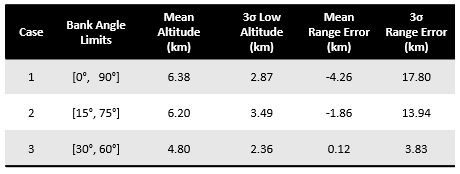
\includegraphics[width=0.65\textwidth]{../PropellantOptimalJournal/ddp/table_deterministic}
	\label{table_deterministic}
\end{table}
\begin{table}[h!]
	\centering
	\caption{The Monte Carlo statistics for cases 4-6, with reference trajectories designed using the proposed method.}
	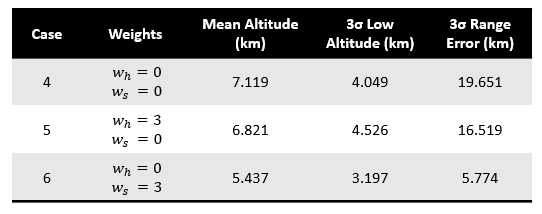
\includegraphics[width=0.65\textwidth]{../PropellantOptimalJournal/ddp/table_robust} %
	\label{table_robust}
\end{table}
%Figures~\ref{fig_robust_alt}-\ref{fig_robust_range} show the estimated $3\sigma$ deviations around the mean as well as the sigma point trajectories for scenario 1.
%\begin{figure}[h!]
%	\centering
%	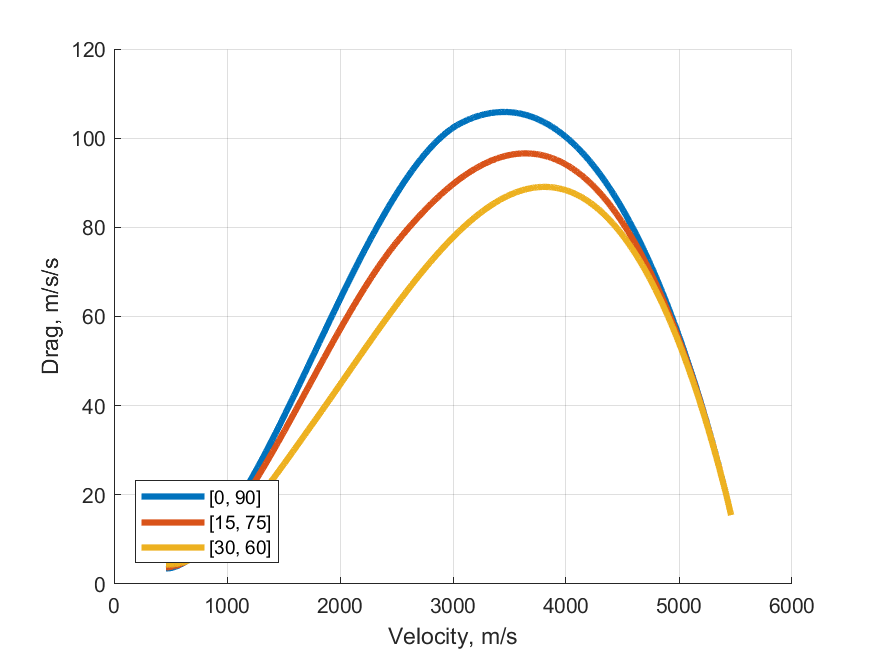
\includegraphics[width=1\textwidth]{ddp/matlab/NominalDrag}
%	\caption{Reference drag profile for each of the four scenarios in Table~\ref{table_comparison}.}
%	\label{fig_drag}
%\end{figure}
%\begin{figure}[h!]
%	\centering
%	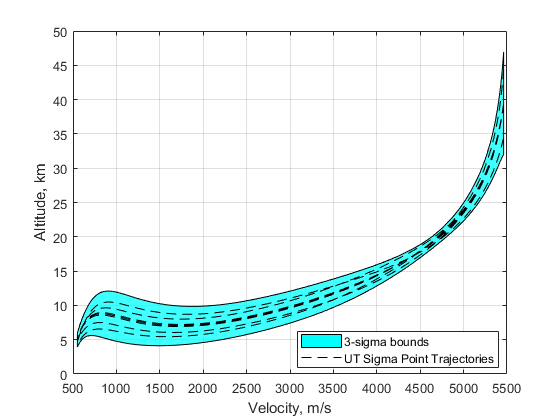
\includegraphics[width=1\textwidth]{ddp/matlab/RobustTrajAlt}
%	\caption{Dispersed altitude performance for scenario 1.}
%	\label{fig_robust_alt}
%\end{figure}
%\begin{figure}[h!]
%	\centering
%	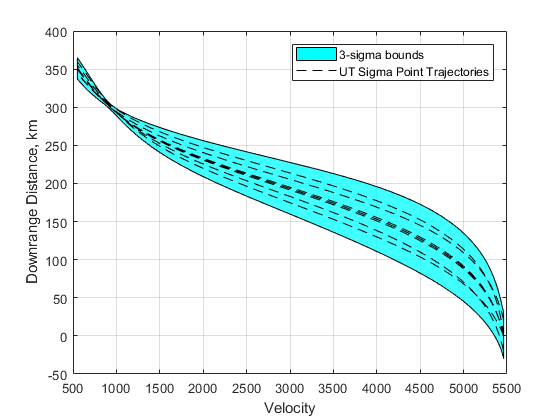
\includegraphics[width=1\textwidth]{ddp/matlab/RobustTrajRange}
%	\caption{Dispersed range performance for scenario 1.}
%	\label{fig_robust_range}
%\end{figure}


\section{Standard Deviation Weighting Design Trade}\label{Sec:HeavyWeightTrade}
%TODO: Double check these numbers, they may have changed 
From the previous subsection it is evident there exists a design space where weights on deviations produce superior results to simply optimizing the mean altitude when tail behavior of the distribution is important. This section investigates the extent to which weighting the standard deviations can alter the trajectory performance. The robust optimal control problem is solved for a variety of weights. The results are summarized in Fig.~\ref{fig_weight_sweep}. Again the advantages of weighting the standard deviations compared with optimizing only the mean are made clear. Comparing $w_h=w_s=0$ with, e.g., $w_h=1,\,w_s = 1$ demonstrates that a 50\% reduction in the standard deviation of downrange distance can be obtained with no loss in the low end of the terminal altitude distribution. Additionally, we can numerically determine the trade between terminal altitude and downrange robustness. The minimum downrange standard deviation achieved ($w_h=1,w_s=3$) was 0.7 km, an 85\% reduction from the mean optimization with $\sigma_s(v_f)=5.1$ km. These trajectories show clear improvements with no change to the guidance gains - simply a different reference trajectory is used to improve the results. The downrange distance shows only small improvement for weights $w_s>1$, but the low altitude continues to drop as this weight is increased. Thus, a compromise such as $w_h=w_s=1$ strikes a good balance between the two objectives. 
\begin{figure}[h!]
	\centering
	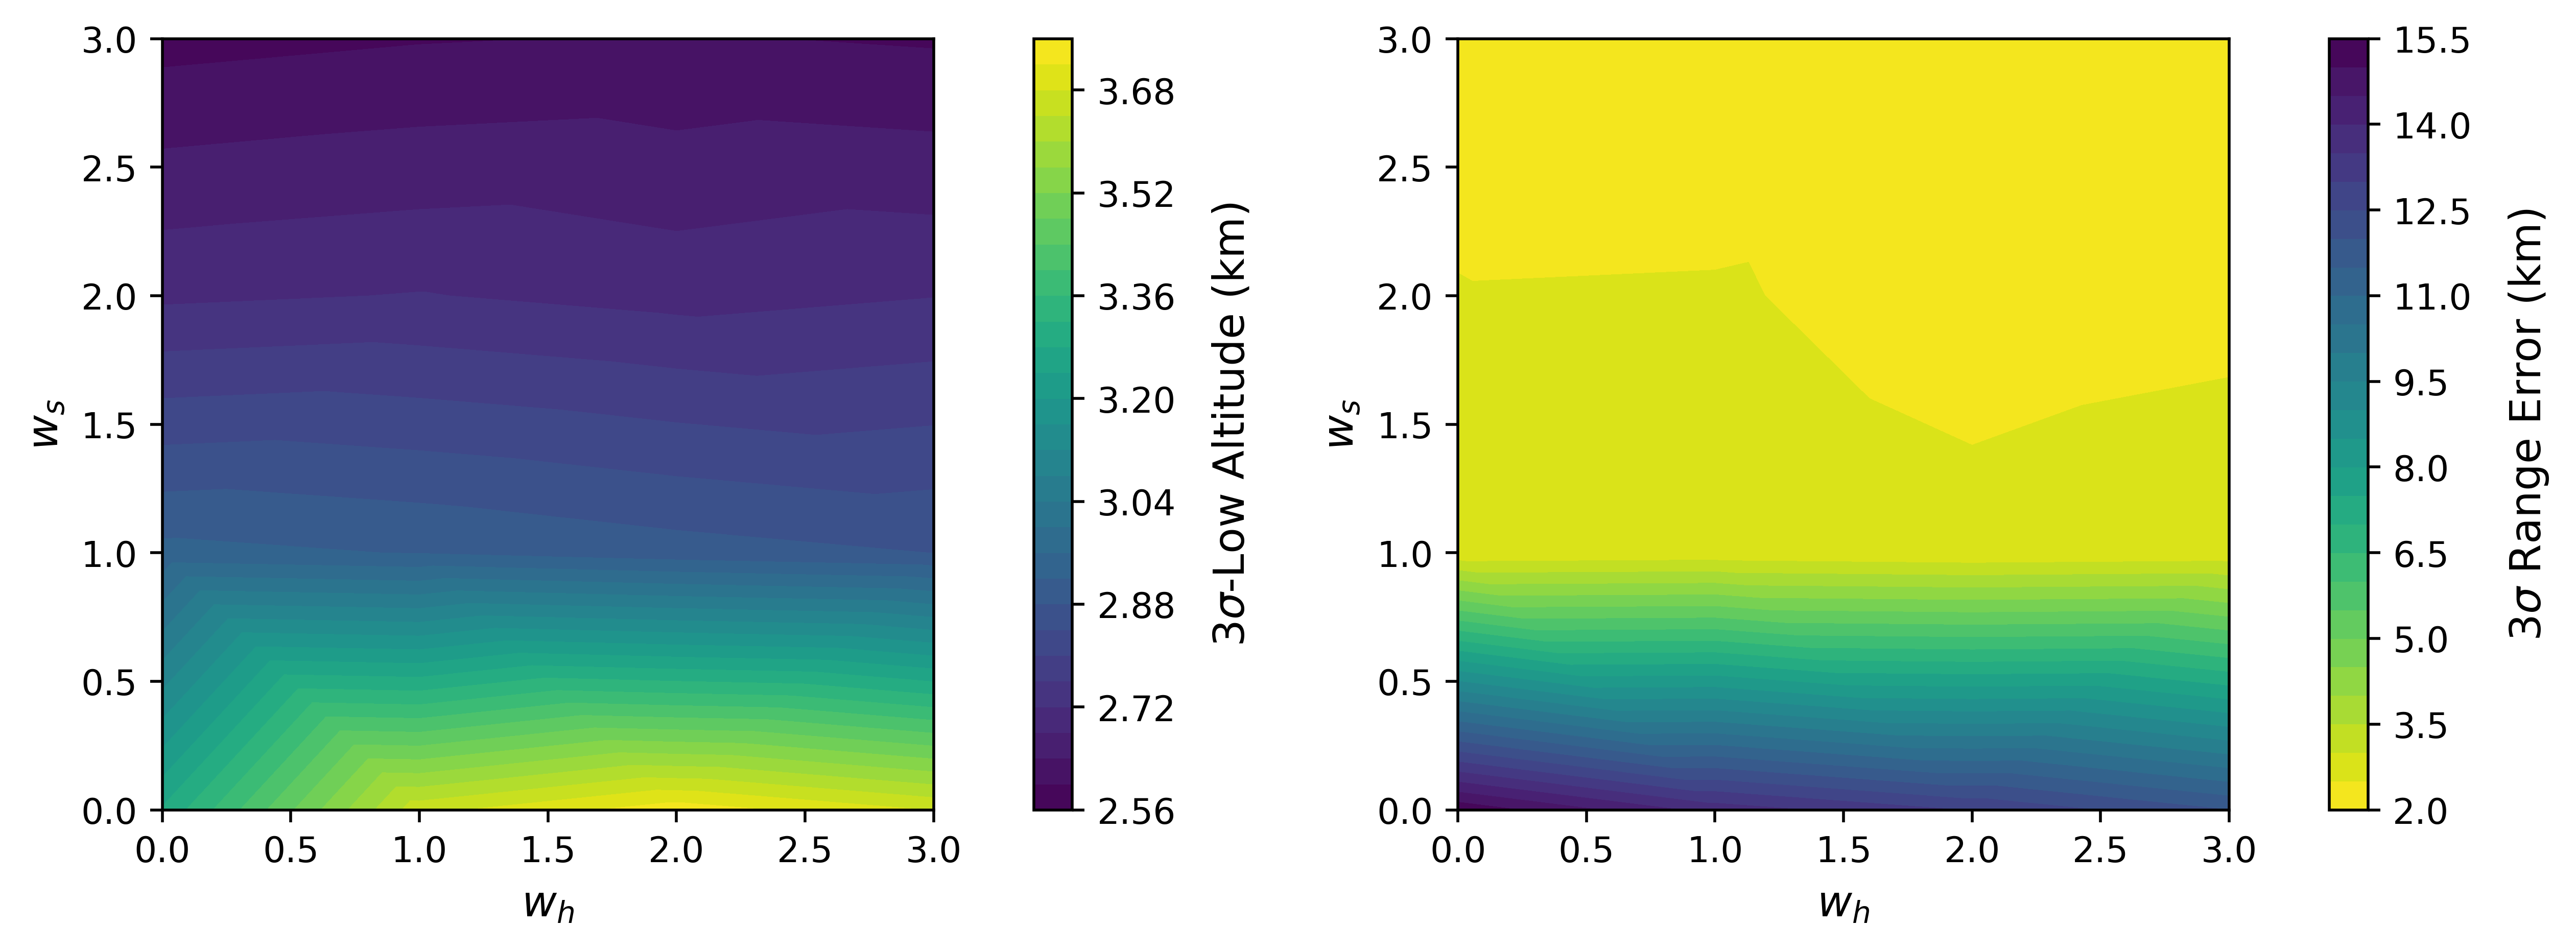
\includegraphics[width=1\textwidth]{../PropellantOptimalJournal/ddp/python/Heavy_WeightSweepMCResults}
	\caption{Contours of the Monte Carlo 3$\sigma$-low altitude (left) and 3$\sigma$ downrange distance error (right) as a function of the weights $w_h$ and $w_s$.}
	\label{fig_weight_sweep}
\end{figure}

These results also show some inaccuracy due to using the unscented transform. The 3$\sigma$-low altitude should be maximized when the objective function is exactly this quantity, i.e., $w_h=3,\,w_s=0$, but due to small estimation errors this is not the case, and the highest 3$\sigma$-low altitude is achieved with $w_h=2,\,w_s=0$. Similarly, the 3$\sigma$ range error is not minimized when $w_h=0,\,w_s=3$, but instead $w_h=1,\,w_s=3$. However, the difference in each of these cases is quite small. This issue is related to that fact that a constant UT scaling parameter $\alpha=15$ is used in all computations. Our experience with the numerical results suggests that the optimal value of $\alpha$ depends on the weights selected, and larger weights should use a higher $\alpha$. 
%Nevertheless, the solutions at all weight values are acceptable
%This also highlights the power of the approach as a design tool. If, for example, the $3\sigma$-low terminal altitude is not sufficient for any values of $w_h,\,w_s$, then some aspect of the mission must be reconsidered: increase the terminal velocity, increase the vehicle $L/D$, decrease ballistic coefficient, etc. If a $3\sigma$-low altitude limit is known, then only points that satisfy this limit are considered, and the point with the lowest downrange error may be selected. 

These results used constant feedback gains, so it is likely that methods of generating gains that vary along the trajectory, such as the Linear-Quadratic Regulator, Apollo influence coefficients \cite{Apollo}, or joint optimization of the feedback gains in the robust optimal control problem, could produce even greater synergistic improvements to the trajectory design. Additionally, the constant feedback gains were optimized for the initial guess trajectory, so further improvement is possible by reoptimizing the gains for the converged trajectory and control, as will be done in the following subsection.

\section{Comparison of UT and Monte Carlo Statistics}
The previous subsections looked at broader trends when using the proposed method to design reference trajectories. This subsection will focus on a single solution, and compare the UT and Monte Carlo statistics in greater detail. Additionally, the feedback gains are again constants, but for this case they are reoptimized to minimize UT-estimated downrange errors after finding the optimal reference control with the previous gains. The reoptimized gains are $[k_D, k_{\gamma}, k_s] = [0.058, -0.021, -0.005]$. Since each component of the objective is important and a compromise must be met, we select the weights $w_h=w_s=1$. A Monte Carlo simulation is conducted with 8000 samples in order generate precise statistics for comparison with the unscented transform. 
\begin{table}[h!]
	\centering
	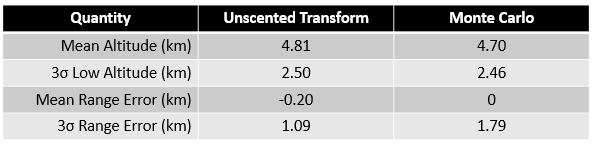
\includegraphics[width=0.75\textwidth]{../PropellantOptimalJournal/ddp/table_mc}
	\caption{Summary of the statistics from the Unscented Transform and Monte Carlo}
	\label{table_mc}
\end{table}
\begin{figure}[h!]
	\centering
	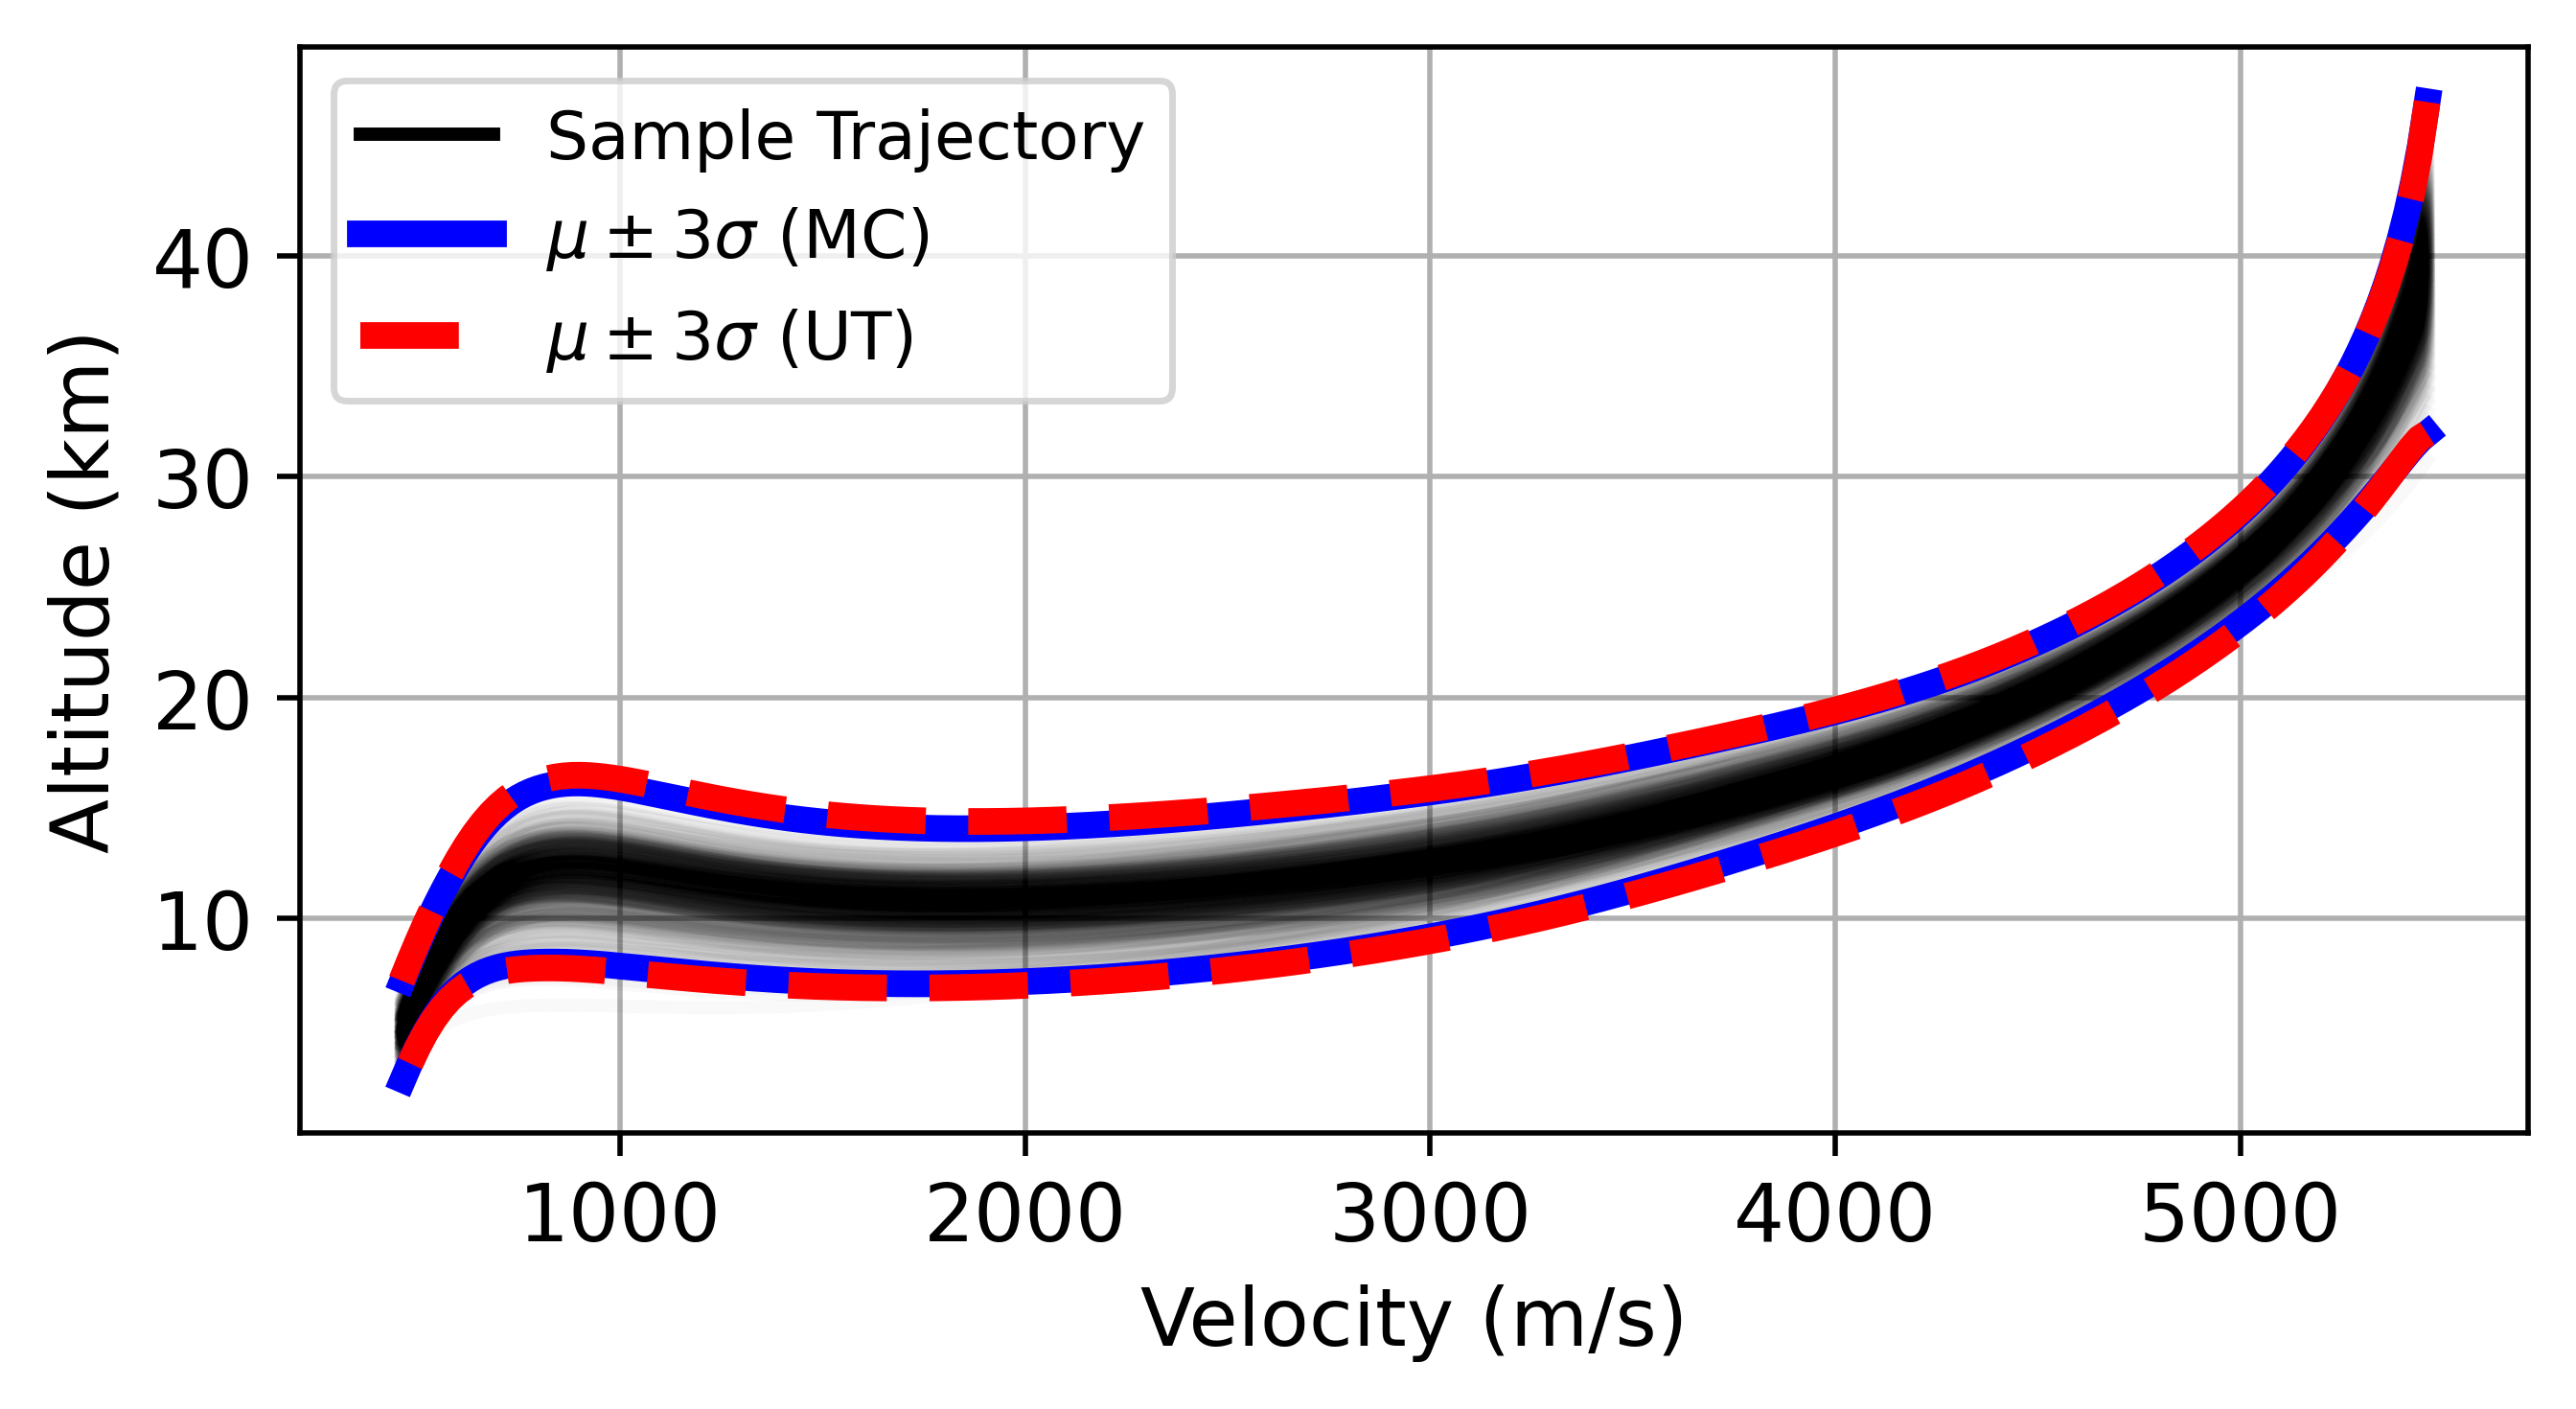
\includegraphics[width=0.75\textwidth]{../PropellantOptimalJournal/ddp/python/Altitude}
	\caption{Altitude versus velocity for 500 sample trajectories with Monte Carlo- and UT-estimated 3$\sigma$ bounds. The 3$ \sigma $-low altitude is 2.5 km.}
	\label{fig_mc_alt}
\end{figure}
\begin{figure}[h!]
	\centering
	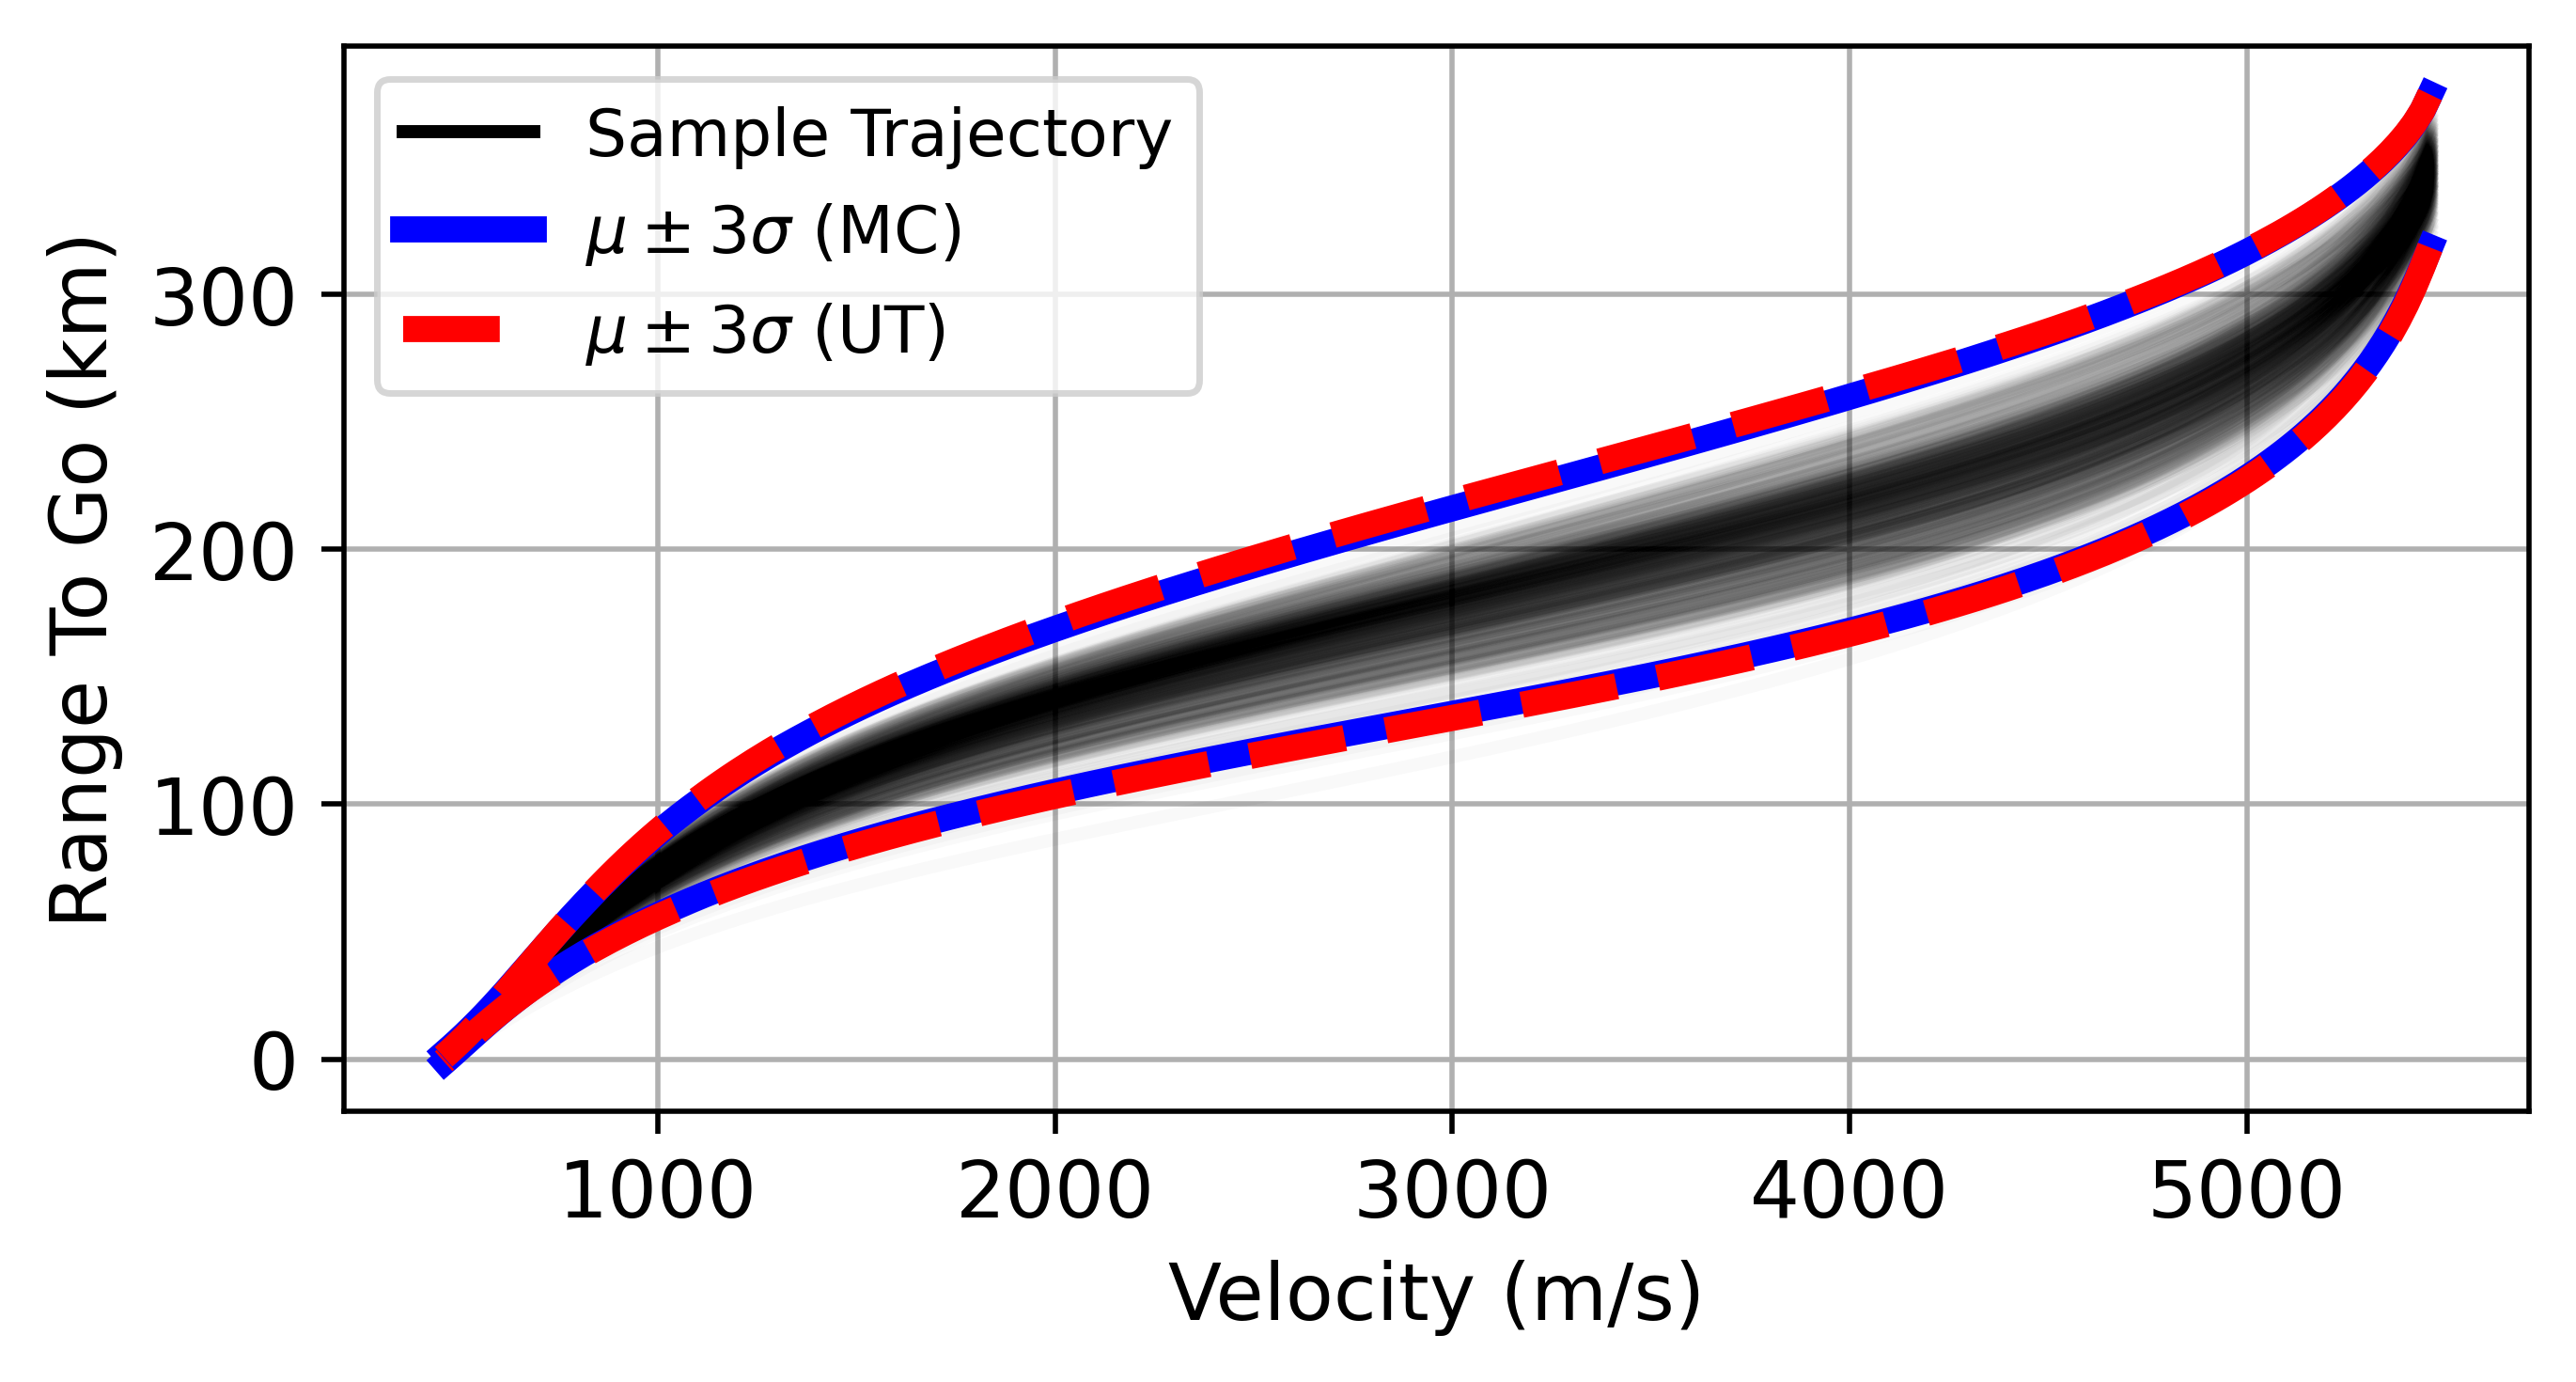
\includegraphics[width=0.75\textwidth]{../PropellantOptimalJournal/ddp/python/Range}
	\caption{Range to go versus velocity for 500 sample trajectories with Monte Carlo- and UT-estimated 3$\sigma$ bounds. The terminal 3$ \sigma $ range error is 1.8 km.}
	\label{fig_mc_range}
\end{figure}
\begin{figure}[h!]
	\centering
	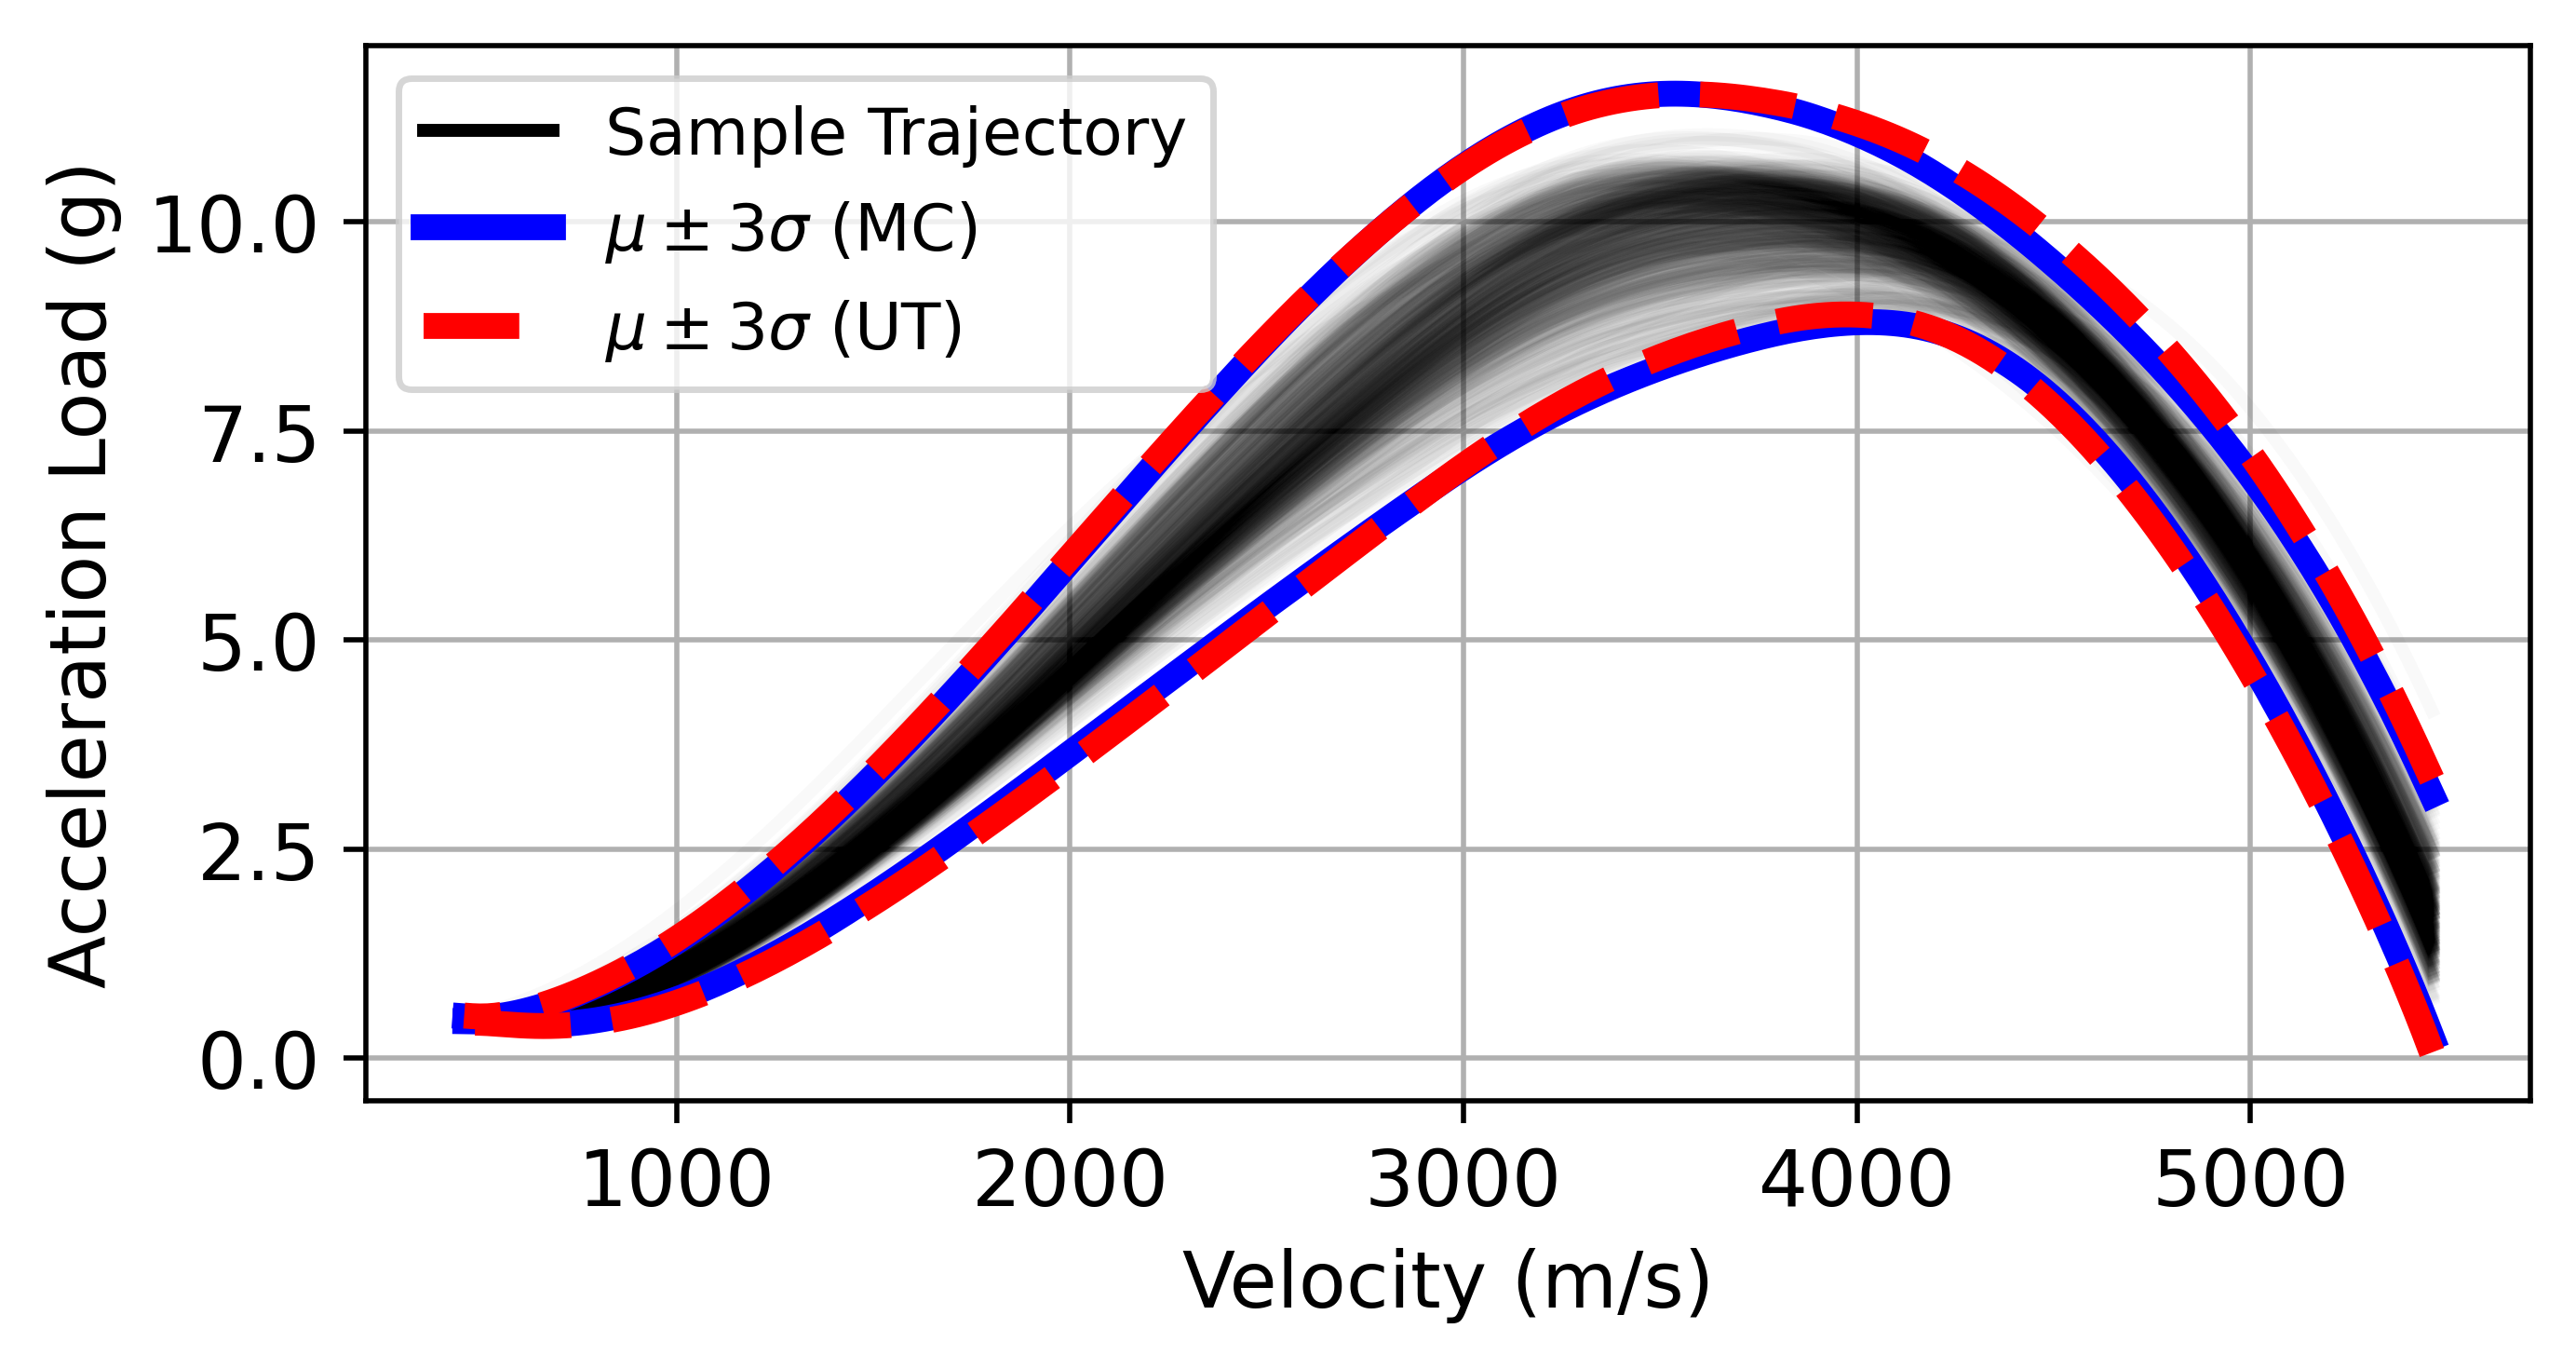
\includegraphics[width=0.75\textwidth]{../PropellantOptimalJournal/ddp/python/Acceleration}
	\caption{Acceleration load vs velocity for 500 sample trajectories with Monte Carlo- and UT-estimated 3$\sigma$ bounds.}
	\label{fig_mc_accel}
\end{figure}
\begin{figure}[h!]
	\centering
	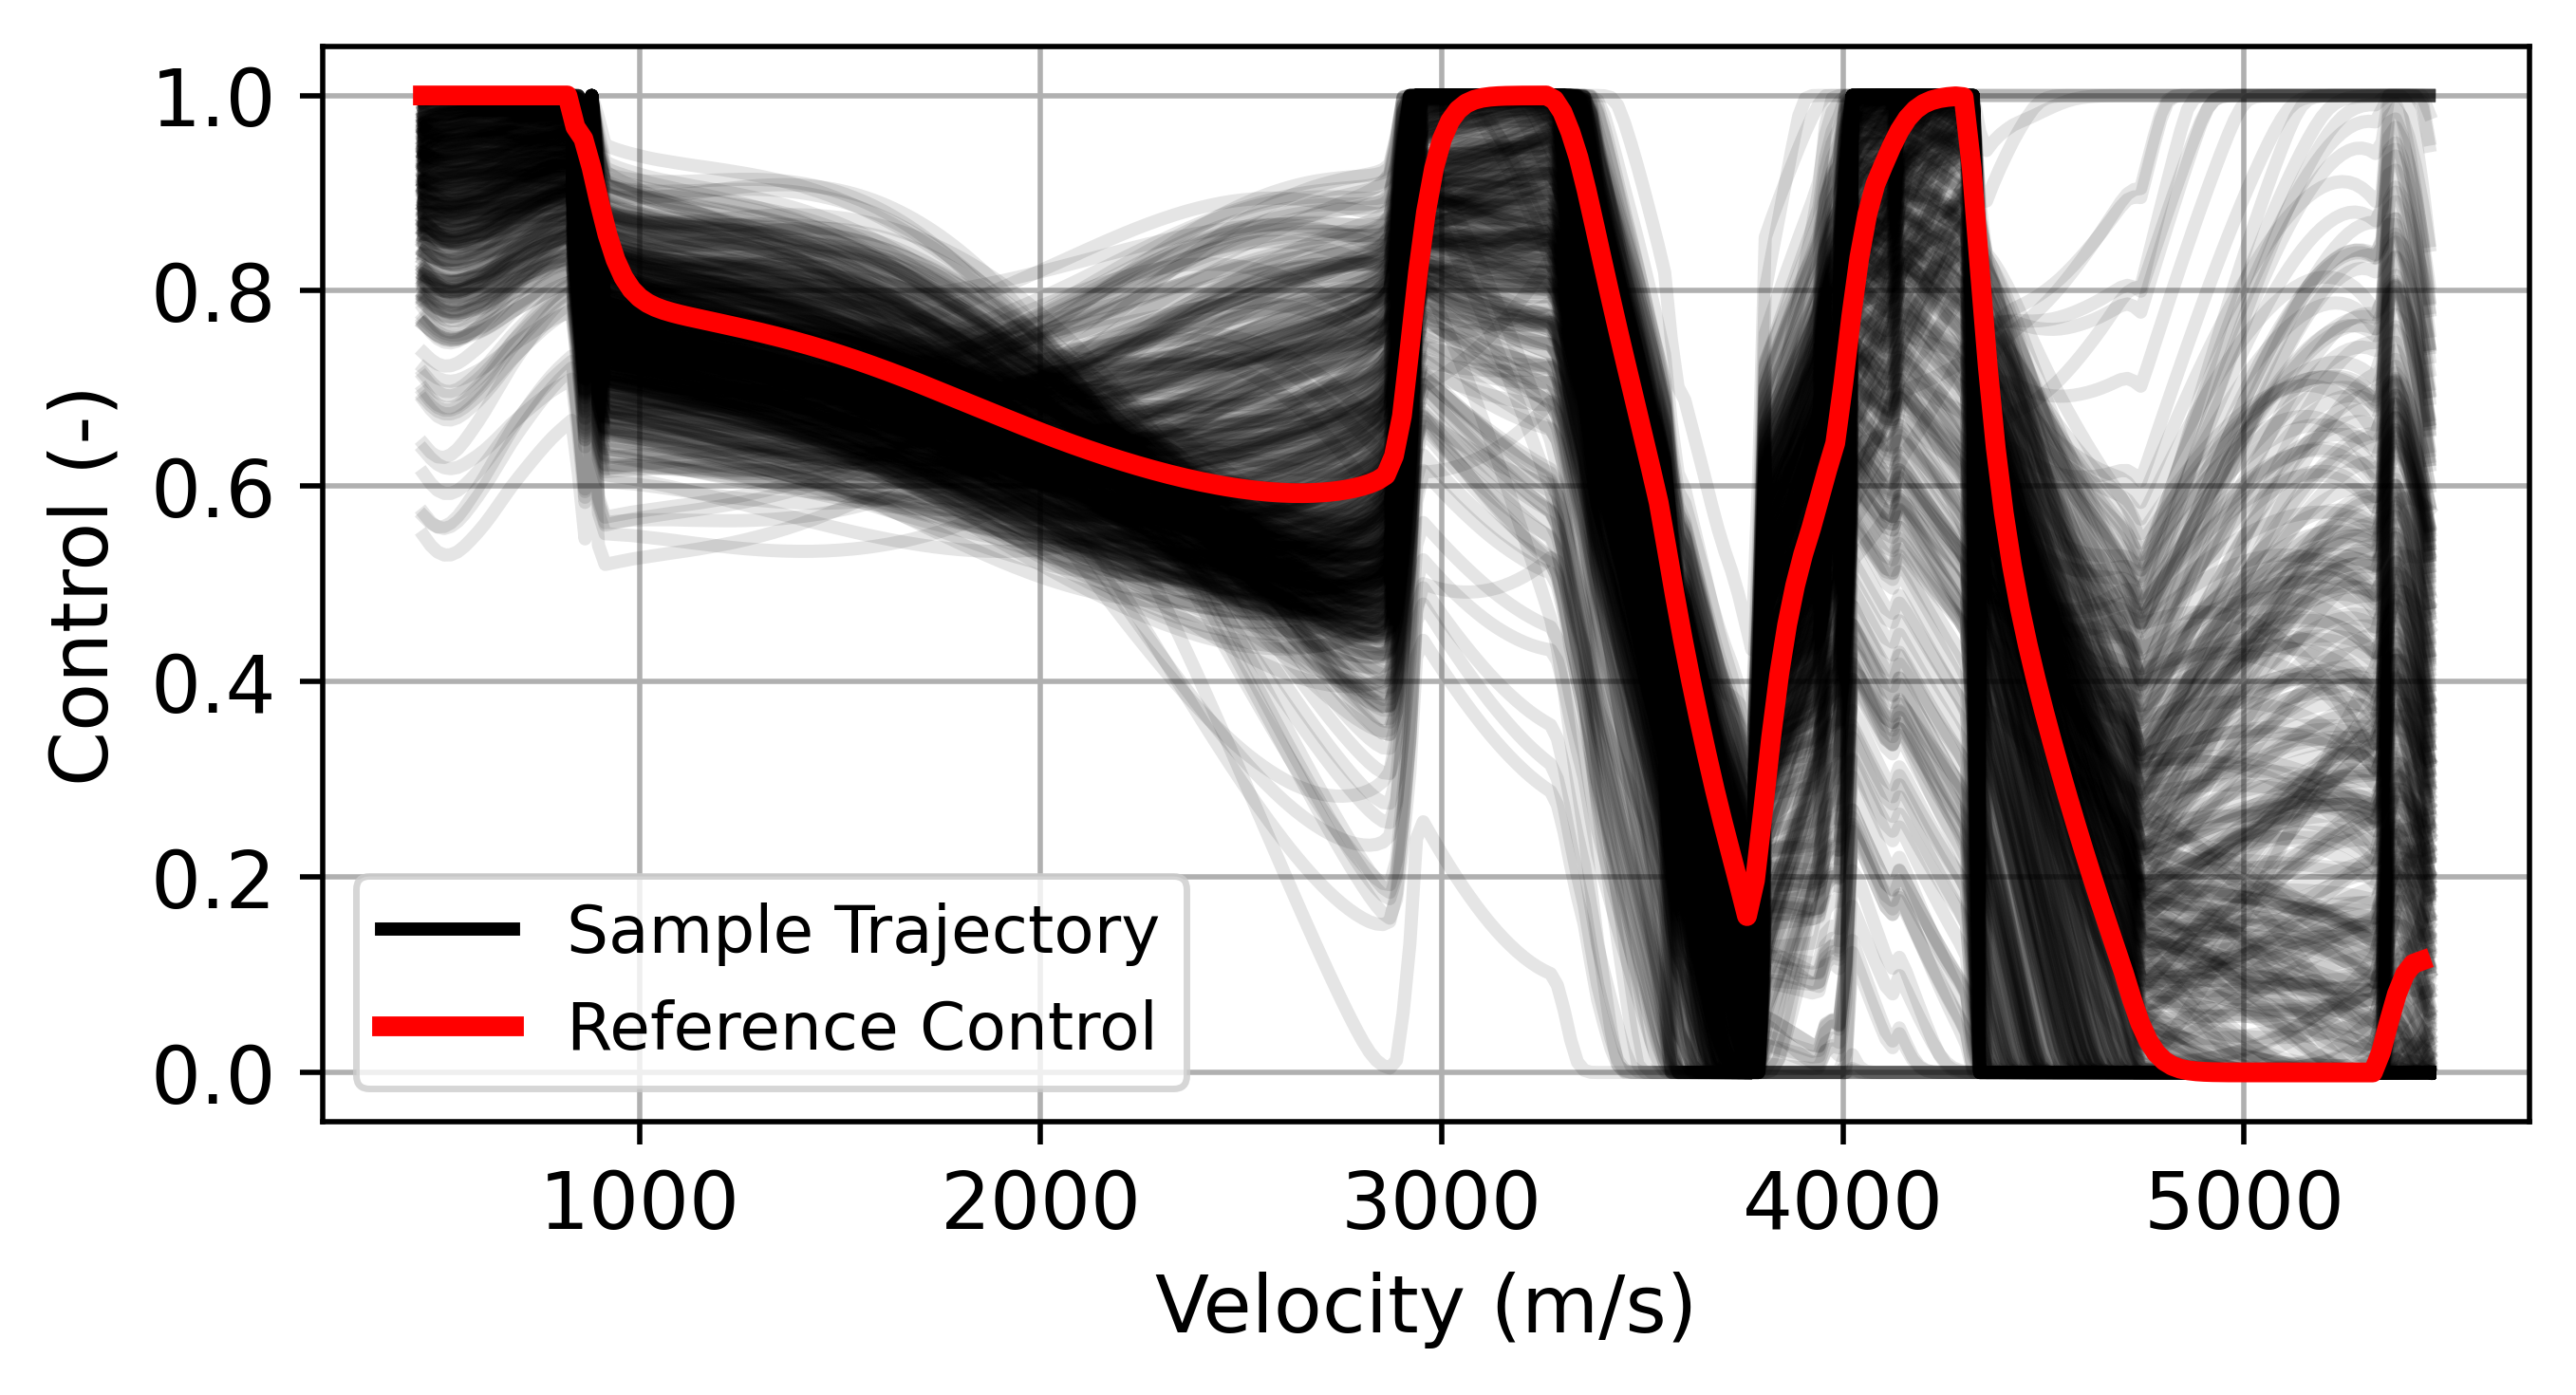
\includegraphics[width=0.75\textwidth]{../PropellantOptimalJournal/ddp/python/Control}
	\caption{The reference control and 500 sample trajectories.}
	\label{fig_mc_control}
\end{figure}
%Reoptimization of the gains resulted in reduction in the 3$\sigma$ range error from 2.5 km to 1.8 km.

% Statistics comparison 
Table~\ref{table_mc} compares statistics estimated with the unscented transform and Monte Carlo simulation. The reference trajectory and constant gains are quite effective, with the Monte Carlo 3$ \sigma $ range error under 2 km, despite small UT-estimation errors. This is achieved in part due to the reoptimization of the gains. This result is further strengthened by comparison with the performance of the unguided vehicle, which we recall was 3$\sigma_s = 80$ km. This is very nearly a 98\% reduction in 3$\sigma$ range error at a cost of 630 meters in 3$\sigma$-low altitude, again compared to the unguided statistics.
Relative to the Monte Carlo results, the UT overestimates the mean altitude by 100 m, the low altitude by 40 m, and underestimates the 3$\sigma $ range error by 700 m, or nearly 40\%. Because the mean trajectory is used as the reference, the UT-estimated mean error is always zero.

Figures~\ref{fig_mc_alt}-\ref{fig_mc_accel} show 500 sample trajectories as well as the Monte Carlo estimated 3$\sigma$ bounds, and the UT-estimated 3$\sigma$ bounds for comparison. Each of these figures demonstrates that the UT-estimated statistics closely approximate the Monte Carlo statistics. Like the terminal statistics in Table~\ref{table_mc}, the UT estimation errors do not have a consistent sign at every point along a trajectory; on some intervals the UT underestimates the 3$\sigma$ bounds, while on other intervals it overestimates them. More importantly, the magnitude of these errors remains small, confirming that the UT is an effective method of quantifying uncertainty in the optimization process. 
% Solution features 
Figure~\ref{fig_mc_alt} shows that lofting at low velocities is a key feature of the trajectories used to raise the terminal altitude. Contrary to prior studies that found range control is not effective at low velocities \cite{MSL_EDL2}, Fig.~\ref{fig_mc_range} shows the convergence of the 3$\sigma$ range errors from 25 km at $ v=1100 $ m/s to less than 2 km at the $v=460$ m/s. 
Figure~\ref{fig_mc_accel} shows the acceleration loads which never exceed 12g. If, as with MSL, a 15g limit is imposed, then this result indicates that a steeper mean entry flight path angle can be accommodated.

Figure~\ref{fig_mc_control} shows the reference control as well as the sample controls for the same 500 trajectory subset. The reference control resembles bang-bang profiles at high velocities before transitioning gradually to a full lift up orientation. There exist intervals with significant margin, particularly between 1000 m/s and 3000 m/s, as well as intervals in which the reference control and many sample controls are saturated. 
This is important because a full lift up orientation leaves no control authority for lateral guidance to manage the vehicle crossrange distance to the target.

%\section{Discussion}
SRL will land near Mars 2020 in Jezero Crater at an altitude of -2.566 km MOLA. The range of altitudes achieved using the method demonstrates that, for the heavier vehicle under consideration, a constant $ L/D=0.28 $ is not sufficient to reach the required altitude. Nevertheless, the  altitude optimal solutions in the second section of this chapter indicate the maximum altitude reachable in the nominal scenario is about 6.4 km, providing a value against which the 3$\sigma$-low altitudes from the robust optimal solutions may be compared. The 3$\sigma$-low altitudes in Section~\ref{Sec:HeavyWeightTrade} ranged from 2.6 km to 3.7 km, or altitude losses of 3.8 km and 2.7 km relative to the maximum altitude trajectories. Case 6 had a 3$\sigma$-low altitude loss of 2.25 km relative to the mean altitude with a tight 3$\sigma$ range error of 2.5 km. 
Overall, the robust optimal solutions for this heavier class of vehicle show similar robustness to the results of the previous chapter for the MSL-class vehicle. 

%Using the robust guidance as a design tool, we can quickly determine what constant (or up scaled MSL profile) L/D would be required to raise the 3$\sigma$-low altitude above 4.566. To bound this value from below, we consider $w_h=3,w_s=0$.

%However, the 3$\sigma$-low altitudes are approximately consistent with a landing at the intended elevation in Jezero Crater where Mars 2020 landed. 

%%% Local Variables: ***
%%% mode: latex ***
%%% TeX-master: "thesis.tex" ***
%%% End: ***
